\documentclass{article}

% PACKAGES
\usepackage[utf8]{inputenc}
\usepackage{hyperref}
\usepackage{listings}
\usepackage{bbding}
\usepackage{float}
\usepackage{graphicx}
%PREAMBOLO
\lstdefinestyle{bashstyle}{
  language=bash,
  basicstyle=\ttfamily,
  numbers=left,
  numberstyle=\tiny,
  numbersep=5pt,
  frame=tb,
  columns=fullflexible,
  showstringspaces=false
}

% TITLE
\title{Prodotto tra una matrice sparsa ed un multivettore}

% AUTHORS
\author{Luca Capotombolo, Ludovico Zarrelli}

%DATE
\date{1 Luglio 2023}

% DOCUMENT
\begin{document}

\maketitle

\tableofcontents

\clearpage

\section{Introduzione}

\subsection{Contesto}
Il progetto prevede la realizzazione di un nucleo di calcolo per il prodotto tra una matrice sparsa ed un multivettore:
\begin{center}
\textit{Y = AX}
\end{center}
dove \textit{A} è una matrice sparsa memorizzata nei formati \textit{CSR} e \textit{ELLPACK}. Il nucleo di calcolo è stato sviluppato in C ed è stato parallelizzato per sfruttare le risorse di calcolo disponibili con parallelizzazione \textit{OpenMP} e \textit{CUDA}. \\

Nel progetto sono state utilizzate le matrici nel formato \textit{MatrixMarket}. Per determinare la tipologia di matrice rappresentata nel file Matrix Market sono state utilizzate le funzioni di I/O disponibili all'indirizzo:
\url{https://sparse.tamu.edu/}

\subsection{Matrici di test}
Per quanto riguarda le matrici di test, sono state scaricate nel formato \textit{Matrix Market} e sono state utilizzate le funzioni per l'I/O disponibili all'indirizzo: \url{http://math.nist.gov/MatrixMarket/}

\subsection{Implementazione Seriale}
I risultati ottenuti dall'esecuzione parallela SpMM sono stati confrontati direttamente con i risultati ottenuti dall'esecuzione seriale. Per quanto riguarda le implementazioni seriali, sono state sviluppate tre differenti versioni:

\begin{itemize}
\item Prodotto seriale utilizzando il formato CSR
\item Prodotto seriale utilizzando il formato ELLPACK con \textit{zero padding}
\item Prodotto seriale utilizzando il formato ELLPACK senza \textit{zero padding}
\end{itemize}

Per avere una misura dell'errore, abbiamo deciso di calcolare due differenti errori che ci forniscono diverse informazioni:
\begin{itemize}
\item \textit{Massimo errore relativo}: mi fornisce delle informazioni su quale sia l'errore relativo più grande tra tutti i confronti elemento per elemento.
\item \textit{Errore relativo medi0}: mi fornisce delle informazioni sulla media degli errori relativi su tutti i confronti elements by elements 
\end{itemize}

Questi valori vanno confrontati con un valore di tolleranza: IEEE unit roundoff per il tipo di dato double, che è $2.2204460492503131e-016$ 

\section{Funzioni ausiliarie per il pre-processamento dei dati}
La funzione \textit{create\_matrix\_coo} ha il compito di leggere i dati da uno specifico file nel formato \textit{MatrixMarket} per poi allocare e popolare la matrice nel formato \textit{COO}. All'interno di questa funzione vengono gestite le possibili tipologie di matrici che sono supportate dal programma:

\begin{itemize}
\item \textit{Simmetrica Pattern}
\item \textit{Simmetrica Reale}
\item \textit{Generale Pattern}
\item \textit{Generale Reale}
\end{itemize}

Le strutture dati che vengono utilizzate per la rappresentazione della matrice \textit{COO} sono le seguenti:

\begin{itemize}
\item \textit{I}: array contenente gli indici di riga degli elementi non zero
\item\textit{J}: array contenente gli indici di colonna degli elementi non zero
\item \textit{val}: array contenente i valori degli elementi non zero
\end{itemize}

In questo modo, l'elemento \textit{i-esimo} di questi tre array rappresenta rispettivamente l'indice di riga, l'indice di colonna e il valore di uno specifico elemento non zero della matrice.

\section{Discussione implementazione CSR}
Passiamo alla discussione relativa al formato CSR. Vedremo gli aspetti riguardanti la conversione della matrice dal formato \textit{COO} al formato \textit{CSR} e gli aspetti che riguardano il prodotto SpMM sia con \textit{OpenMP} che con \textit{CUDA}.

\subsection{Funzioni ausiliarie per la memorizzazione nel formato CSR}
Le strutture dati che vengono utilizzate per il formato \textit{CSR} sono le seguenti:

\begin{itemize}
\item \textit{as}: è l'array dei coefficienti non zero
\item \textit{ja}: è l'array degli indici di colonna dei coefficienti non zero
\item \textit{irp}: è l'array dei puntatori all'inizio di ciascuna riga
\end{itemize}

Durante lo sviluppo del progetto, abbiamo avuto dei problemi nella conversione della matrice dal formato \textit{COO} al formato \textit{CSR}. Più precisamente, le nostre difficoltà erano dovute al grande tempo richiesto per eseguire la conversione per le matrici di grande dimensione.\\
La prima implementazione dell'algoritmo di conversione è rappresentata dalla funzione \textit{coo\_to\_CSR\_parallel} che si comporta bene per le matrici di piccole/medie dimensione ma ha un tempo di esecuzione elevato per la matrici di grande dimensione. Il primo step dell'algoritmo consiste nel computare il numero di non zeri per ogni riga popolando la struttura dati di appoggio \textit{nz\_per\_row} che poi viene utilizzata per inizializzare la struttura dati \textit{irp}. A questo punto, le tre strutture dati precedentemente elencate vengono popolate utilizzando un doppio ciclo \textit{for}. Per velocizzare l'esecuzione, questo blocco di codice è stato parallelizzato cercando di bilanciare il più possibile il carico di lavoro. Per liberare la memoria precedentemente occupata, al termine dell'inizializzazione delle tre strutture dati \textit{as, ja} e \textit{irp} vengono deallocate le strutture dati per la rappresentazione nel formato \textit{COO}. \\
Il problema della prima implementazione è rappresentato dalla presenza dei due cicli for, che comporta un numero di iterazioni pari a M * nz, dove M è il numero di righe e nz è il numero complessivo di non zeri della matrice in input. Per ridurre il tempo richiesto nella conversione dal formato \textit{COO} al formato \textit{CSR}, in modo da trattare anche le matrici molto grandi, abbiamo deciso di implementare una seconda versione dell'algoritmo di conversione nella funzione \textit{coo\_to\_CSR\_parallel\_optimization}. Il vantaggio di questa seconda versione consiste nell'utilizzo di un singolo ciclo che va ad iterare su tutti i non zeri della matrice. Per gestire la concorrenza, abbiamo introdotto una minima sezione critica che, comunque, ci consente di avere dei tempi di esecuzione molto inferiori rispetto alla versione precedente.

\subsection{OpenMP}
Il prodotto parallelo per il formato \textit{CSR} con parallelizzazione \textit{OpenMP} è implementato nella funzione \textit{parallel\_product\_CSR}. La funzione \textit{compute\_chunk\_size} ha il compito di calcolare la dimensione del chunk che deve essere assegnato a ciascun thread. Lo spazio delle iterazioni viene suddiviso a seconda del numero di processori che sono disponibili sul device. 
Inoltre, per evitare il false cache sharing, il valore $ \frac {Numero\_di\_iterazioni} {Numero\_di\_processori} $ è arrotondato all'intero più vicino (inferiore) multiplo di 16.
L'obiettivo è quello di assegnare un blocco di righe contiguo ai threads nello spazio di iterazione in modo da evita il più possibile il problema del \textit{False Cache Sharing}. Ad ogni thread viene associato un certo numero di righe e ogni riga è associata ad un unico thread. In questo modo, posso utilizzare una variabile privata \textit{partial\_sum} per computare le somme parziali. Abbiamo scelto la clausola static perché abbiamo assunto che ogni iterazione abbia un costo per lo più costante.

\subsection{CUDA}
Per quanto riguarda il prodotto parallelo per il formato \textit{CSR} in \textit{CUDA}, abbiamo deciso di scrivere differenti versioni del kernel. In realtà, le prime tre versioni del kernel potrebbero essere viste come la stessa versione con solamente delle modifiche minimali che le distinguono. Abbiamo deciso di riportare queste modifiche minimali differenziando così le tre versioni del kernel poiché hanno un grande impatto prestazionale. Poiché stiamo facendo calcolo ad alte prestazioni, è importante notare come queste differenze, che sembrano essere minimali, in realtà hanno un gran peso sulle prestazioni.\\
L'idea che c'è dietro alle prime tre versioni del kernel è quella di far sì che un singolo thread computi un singolo elemento della matrice finale \textit{Y}. Inizialmente, viene allocata la memoria necessaria sul \textit{CUDA Device} e vengono copiati i dati dall'host verso il device. Il numero di threads per blocco che viene utilizzato è pari a \textit{512} (Alcune prove empiriche hanno rivelato un miglioramento delle performance per un numero di threads per blocco pari a 512). Nel kernel vengono calcolati gli indici di riga e di colonna che identificano l'elemento che deve essere calcolato dal thread. Come primo step viene calcolato l'identificativo globale del thread. Successivamente, vengono calcolati i due indici nel seguente modo:

\begin{center}
\item \textit{row = tid / K}
\item \textit{col = tid \% K}
\end{center}

Una volta determinata la riga \textit{row} della matrice sparsa \textit{A} e la colonna \textit{col} della matrice densa \textit{X}, viene eseguito un controllo per verificare se il thread sta calcolando effettivamente un elemento della matrice. Questo controllo mi consente di gestire una griglia di blocchi che ha un numero totale di threads strettamente maggiore del numero di elementi della matrice che bisogna calcolare.\\
La prima versione del kernel non è ottimizzata poiché nel calcolo del singolo prodotto scalare si accede in memoria ogni volta che il thread modifica il risultato intermedio. Questi accessi continui portano a delle prestazioni molto basse. Un modo evidente per risolvere questo problema prestazionale consiste nello scrivere in memoria direttamente il risultato finale della computazione rappresentato dal valore della variabile \textit{partial\_sum}. Questa modifica permette di aumentare notevolmente le prestazioni del prodotto parallelo. A questo punto, è stata apportata un'ulteriore modifica minimale che consiste nel pre-computarsi le due variabili \textit{start} e \textit{end} e successivamente eseguire il ciclo. La terza versione riesce a guadagnare in termini prestazionali rispetto alla seconda versione.\\

Dopo aver implementato queste tre versioni del kernel abbiamo provato a distribuire la computazione richiesta per il calcolo di un singolo elemento della matrice. Questa quarta versione è stata ispirata al \textit{CSR Vector} descritto nei vari paper. L'idea è quella di distribuire il calcolo di un elemento della matrice finale Y tra i threads di uno stesso warp. Più precisamente, ogni thread in un warp computa un risultato parziale per uno stesso elemento \textit{y} della matrice \textit{Y}. Viene eseguita una riduzione parallela che coinvolge i thread di uno stesso warp sfruttando la \textit{shared memory}. Poiché tutti i threads di un warp contribuiscono al calcolo dello stesso elemento, è sufficiente che un solo thread tra essi scriva il risultato ottenuto dalla riduzione in memoria globale. Per fare ciò, abbiamo deciso che solamente il thread con identificativo \textit{0} all'interno del warp ha il compito di scrivere il risultato in memoria globale. Tuttavia, questa nuova versione del kernel ci ha portato ad una notevole riduzione delle prestazioni. Il motivo per cui le prestazioni si sono ridotte così drasticamente è dovuto al numero molto piccolo di non zeri per riga. Facendo un'analisi generale delle matrici di test, abbiamo potuto osservare come gran parte di esse abbiano un numero di non zeri medio che è inferiore rispetto alla dimensione del warp. Questo implica il fatto che ci siano mediamente un numero non piccolo di thread all'interno di un warp che non danno un contributo effettivo al calcolo dell'elemento. \\
Un altro fattore impattante è sicuramente il numero di accessi in memoria condivisa. Rispetto alle tre versione di kernel, descritte in precedenza, abbiamo lo stesso numero complessivo di accessi in memoria globale per calcolare le somme parziali, ma abbiamo un notevole numero di accessi in memoria condivisa per realizzare la riduzione parallela e la scrittura finale in memoria globale.
\\

Nelle prime tre versioni, ogni elemento veniva computato da un singolo thread che eseguiva il prodotto scalare riga \textit{row} per colonna \textit{cols}. Nella versione successiva, invece di utilizzare un unico thread, abbiamo provato a distribuire la computazione tra i differenti thread di uno stesso warp. Tuttavia, abbiamo visto che assegnando un singolo warp alla computazione di un singolo elemento \textit{y} della matrice finale \textit{Y} si ha una grande perdita nelle prestazioni. A questo punto, abbiamo pensato di seguire un approccio intermedio che consiste nel vedere i due casi implementati finora come dei \textit{casi estremi}. Invece di assegnare un thread per elemento o un warp per elemento abbiamo provato a scegliere un numero intermedio di thread come compromesso tra i due differenti approcci.\\

Più precisamente, dato un \textit{warp} di 32 thread, abbiamo creato 16 differenti \textit{sub-warp}, ognuno con il compito di computare un singolo elemento della matrice finale \textit{Y}. Di conseguenza, ogni elemento \textit{y} della matrice finale \textit{Y} è computato da due differenti thread (è un valore arbitrario che abbiamo scelto dopo un'attenta analisi empirica delle prestazioni al variare del numero di threads per ogni sub-warp) che costituiscono il sub-warp. Nella versione \textit{CSR\_Vector\_Sub\_warp} si ragiona in termini di identificativo del sub-warp. Come primo step si determina l'identificativo globale del thread per poi computare l'identificativo globale del \textit{sub-warp} a cui il thread appartiene. Poiché un \textit{sub-warp} ha una dimensione pari a \textit{2}, ogni thread che appartiene al \textit{sub-warp} ha un proprio identificativo locale al suo interno. Più precisamente, se la dimensione è pari a \textit{2} allora i possibili indici dei threads all'interno di un sub-warp sono \textit{0} e \textit{1}. Dopo aver calcolato l'indice del sub-warp è possibile determinare la riga e la colonna dell'elemento della matrice assegnato al sub-warp. Poiché il sub-warp si occupa di computare le somme parziali per un singolo elemento della matrice \textit{Y} allora possiamo utilizzare direttamente una sola area di memoria associata ad ogni thread. Da notare che questo non sarebbe stato possibile se il sub-warp avesse calcolato più elementi distinti della matrice finale \textit{Y}. In questo caso, sarebbe stato necessario un meccanismo che permettesse di distinguere le somme parziali per i differenti elementi. In questo kernel viene utilizzata la \textit{shared memory} per mantenere i risultati delle somme parziali. Più precisamente, ad ogni thread viene assegnata una specifica entry nell'array \textit{vals} in cui mantenere i risultati delle somme parziali per il calcolo dell'elemento. Dopo aver calcolato i propri contributi, viene eseguita una riduzione parallela nella memoria condivisa. Infine, solamente il thread con indice \textit{0} all'interno del sub-warp scriverà il risultato in memoria globale. \\

Come suggerito dalla traccia del progetto, abbiamo provato ad implementare anche l'algoritmo \textit{CSR-Adaptive}, ideato per spMV, ma opportunamente adattato per spMM. Per prima cosa vengono individuati i blocchi di righe, in modo tale che per ogni blocco sia assegnata una quantità di memoria condivisa al più pari a \textit{local\_size} (Numero medio di non-zeri per riga) * sizeof(double). Ovviamente, \textit{local\_size} è limitato a 1024, che moltiplicato per 8, è minore di 49152, la quantità totale di memoria condivisa per blocco in bytes dichiarata nella scheda tecnica della GPU. Successivamente, viene invocato il kernel \textit{CSR\_Adaptive} con un numero di blocchi per griglia pari a (numero di blocchi di righe - 1) * K e un numero di threads per blocco pari a \textit{local\_size}. Essendo la memoria condivisa limitata a \textit{local\_size} double non ha senso assegnare piu thread, di questo valore, per blocco. La parte complessa nella "conversione" da algoritmo per spMV a spMM è stata necessità di estenderlo in modo tale da calcolare i prodotti per le restanti K - 1 colonne della matrice \textit{X}. Notare che, rispetto alla versione originale. abbiamo un numero di blocchi per griglia che è K volte più grande. Infatti, l'idea è di avere un blocco che calcola un solo elemento della matrice risultante \textit{Y}. La riga e la colonna da assegnare al blocco corrente sono calcolare nel seguente modo:
    \begin{center}
    \item \textit{row = d\_rowBlocks[ $\frac{blockIdx.x} {K}$ ]} con
    d\_rowBlocks array contenente l'indice della riga iniziale per ogni blocco  
    \item \textit{col = $blockIdx.x \% K$}
    \end{center}

\textit{CSR-Adaptive} è un algoritmo che decide dinamicamente se utilizzare \textit{CSR-Stream}, quando il numero di righe per blocco $>$ 1 o \textit{CSR-Vector}, quando il numero di righe per blocco di righe per blocco pari a 1. \\
\textit{CSR-Stream} si basa sulla seguente idea: ogni thread del blocco scrive in memoria condivisa la componente parziale, di sua competenza, del prodotto finale. Per esempio il thread i del blocco j calcola il prodotto tra $as[irp[row] + i] * X[(j \% K ) * N + ja[irp[row]+ i]$. Successivamente, un numero di threads pari al numero di righe per il blocco corrente eseguono la riduzione scalare dalla memoria condivisa per calcolare l'output finale. 
\\ In questo kernel per sfruttare maggiormente i dati in cache, la matrice \textit{X} è stata trasposta in modo tale che gli elementi della colonna siano contigui in memoria.\\

Anche in questo caso, non soddisfatti delle prestazioni ottenute abbiamo realizzato le seguenti versione ottimizzate per spMM di CSR-Vector e CSR-Adaptive:
  \begin{itemize}
   \item \textit{CSR\_Vector\_by\_row}: 
    Ogni warp, suddiviso in 8 sub-warp, è responsabile del calcolo di tutti le componenti di una riga della matrice risultante. Ogni blocco ha 512 thread, di conseguenza si hanno 16 warp per blocco che in parallelo calcolano 16 righe della matrice Y. Di conseguenza, il numero di blocchi per griglia è pari a $\frac{M}{16}$ con M numero di righe di A e 16 il numero di warp per blocco. I thread del sub-warp collaborano per calcolare un elemento in \textit{Y}, la cui riga è determinata dall' identificativo del warp di cui il sub-warp fa parte. Attraverso la memoria condivisa i thread della prima metà del sub-warp eseguono una riduzione parallela. In breve, abbiamo 8 sub-warp di 4 thread per ogni warp, che si suddividono le K colonne di \textit{X} per calcolare la riga i-esima di \textit{Y}.
   
   \item \textit{CSR\_Adaptive\_sub\_blocks}: Ogni blocco di thread, suddiviso in un certo numero di sub-block, calcola tutte le componenti di una riga della matrice Y. Ogni sub-block di sub\_block\_size thread è responsabile del calcolo di una prodotto della componente di sua competenza per la riga i nella matrice \textit{Y}. Di conseguenza, i thread dello stesso sub-block collaborano tra di loro per calcolare l'output finale.
   \end{itemize}
   
In entrambi i casi la matrice X è stata trasposta in modo tale che gli elementi della colonna siano contigui in memoria. \\

In questo modo abbiamo ridotto il numero di conflitti sulla gerarchia di cache per l'accesso alle colonne della matrice X. Di fatto, abbiamo meno threads che possono accedere in concorrenza alla stessa colonna della matrice X.


\section{Discussione implementazione ELLPACK}
Passiamo alla discussione relativa al formato ELLPACK. Vedremo gli aspetti riguardanti la conversione della matrice dal formato \textit{COO} al formato \textit{ELLPACK} e gli aspetti che riguardano il prodotto SpMM sia con \textit{OpenMP} che con \textit{CUDA}.

\subsection{Funzioni ausiliarie per la memorizzazione nel formato ELLPACK}
Le strutture dati che vengono utilizzate per il formato \textit{ELLPACK} sono le seguenti:

\begin{itemize}
\item \textit{values}
\item \textit{col\_indices}
\end{itemize}

Similmente a quanto descritto nella sezione relativa al formato \textit{CSR}, per rendere più efficiente la convesione della matrice dal formato \textit{COO} al formato \textit{ELLPACK} abbiamo implementato tre differenti versioni per l'algoritmo di conversione che si differenziano per il tempo di esecuzione.\\

La prima versione dell'algoritmo di conversione è stata implementata nella funzione \textit{coo\_to\_ellpack\_parallel()}. In questa prima versione, viene utilizzato il \textit{padding 0x0} per il formato \textit{ELLPACK}. Come primo step viene calcolato il massimo numero degli elementi non-zero \textit{max\_so\_far} tra tutte le righe della matrice sparsa. Dopo aver calcolato il massimo numero di non zeri per riga vengono allocate le strutture dati \textit{values} e \textit{col\_indices}. A questo punto, si passa con il popolare i due array bidimensionali con i valori che si trovano nelle strutture dati \textit{J} e \textit{val} del formato \textit{COO}. Più precisamente, fissata la riga \textit{i-esima} assegnata ad un thread \textit{T}, vengono identificati tutti quanti gli elementi non-zero appartenenti a quella riga e popolo le strutture dati \textit{values} e \textit{col\_indices} con rispettivamente il valore e l'indice di colonna dell'elemento non-zero.\\

Con la prima versione dell'algoritmo di conversione abbiamo riscontrato dei problemi di memoria (\textit{Out Of Memory}) durante l'esecuzione del programma sulle nostre macchine. Per poter eseguire il programma in locale abbiamo deciso di implementare un'altra versione dell'algoritmo di conversione. La seconda versione ha l'obiettivo di risparmiare memoria nella memorizzazione della matrice nel formato \textit{ELLPACK}. Più precisamente, abbiamo deciso di non utilizzare il \textit{padding 0x0} e di gestire le strutture dati \textit{values} e \textit{col\_indices} non necessariamente come tipici array bidimensionali. In questa versione, abbiamo calcolati il numero degli elemento non-zero all'interno di ciascuna riga della matrice popolando il vettore \textit{nz\_per\_row}.\\

Tuttavia, sebbene la seconda versione ci ha permesso di risparmiare memoria aggirando il problema dell'esecuzione locale, entrambe le versioni precedenti richiedono tanto tempo per la conversione dal formato \textit{COO} al formato \textit{ELLPACK} delle matrici di grande dimensioni. Per scavalcare quest'ultimo ostacolo, abbiamo deciso di implementare una terza versione dell'algoritmo di conversione che ci permettesse di eseguire la conversione in un tempo ragionevole per una qualsiasi matrice di test richiesta per il progetto.\\

La terza versione dell'algoritmo di conversione mantiene l'idea di non utilizzare lo \textit{zero padding} per ridurre la quantità di memoria utilizzata. Il primo step consiste sempre nel computarsi il numero di non zeri per riga popolando la struttura dati \textit{nz\_per\_row}. A questo punto, invece di eseguire due cicli for annidati (procedimento adottato nelle precedenti due versioni dell'algoritmo di conversione) si sfrutta un singolo ciclo for con una piccola sezione critica al suo interno. La sezione critica mi consente di evitare un ulteriore ciclo e, nel complesso, di ridurre il tempo di esecuzione per la conversione. Nelle precedenti versioni, un solo thread si occupava della singola riga e lo spazio delle iterazioni era l'insieme delle righe. Nella terza versione, viene partizionato lo spazio degli elementi in modo che gli elementi di una singola riga possano essere assegnati a thread differenti. Viene utilizzata la struttura dati \textit{curr\_idx\_per\_row} che mantiene le informazioni relative all'indice attuale per le varie righe. Questa informazione è necessaria da mantenere poiché più thread possono agire lavorare su una stessa riga.

\subsection{OpenMP}
Il prodotto parallelo per il formato \textit{ELLPACK} con parallelizzazione \textit{OpenMP} è implementato nelle seguenti due funzioni:

\begin{itemize}
\item \textit{parallel\_product\_ellpack()}
\item \textit{parallel\_product\_ellpack\_no\_zero\_padding()}
\end{itemize}

Nel prodotto parallelo con \textit{ELLPACK} abbiamo deciso di utilizzare la trasposta della matrice \textit{X} che viene calcolata tramite la funzione \textit{transpose}. Per quanto riguarda la distribuzione del carico di lavoro tra i vari thread, abbiamo deciso di utilizzare la clausola \textit{schedule} con \textit{static}. In questo modo, le iterazioni del ciclo sono divise in parti con dimensione pari a \textit{chunk\_size} e sono staticamente assegnati ai thread. Il valore di \textit{chunk\_size} viene calcolato considerando il numero \textit{M} di righe della matrice e il numero di processori \textit{ntherad} disponibili sul dispositivo. L'idea è quella di distribuire le righe della matrice tra i vari thread che sono disponibili per l'esecuzione. Inoltre, utilizziamo anche la clausola \textit{collapse} poiché abbiamo due differenti cicli innestati perfettamente (il ciclo che itera su \textit{M} e quello che itera su \textit{K}). La differenza tra le due funzioni \textit{parallel\_product\_ellpack()} e \textit{parallel\_product\_ellpack\_no\_zero\_padding()} sta nella gestione delle righe poiché la versione senza \textit{zero padding} utilizza strutture dati leggermente differenti. Infatti, nella versione che utilizza il padding il ciclo for più interno itera fino al numero massimo di non zeri per riga mentre nella versione ottimizzata si itera fino alla dimensione effettiva di quella riga che ottengo tramite la struttura dati \textit{nz\_per\_row}.

\subsection{CUDA}
Per quanto riguarda il prodotto parallelo per il formato \textit{ELLPACK} in \textit{CUDA}, abbiamo deciso di implementare due differenti versioni del kernel:

\begin{itemize}

\item \textit{ELLPACK\_kernel}:
    L'idea di far sì che un singolo thread computi un singolo elemento della matrice finale \textit{Y}. Anche in questo caso il numero di thread per blocco che viene utilizzato è pari a \textit{512}.
    Nel kernel vengono calcolati gli indici di riga e di colonna che identificano l'elemento che deve essere calcolato dal thread:

    
\begin{center}
\item \textit{row = tid / K}
\item \textit{col = tid \% K}
\end{center}

    Una volta determinata la riga \textit{row} della matrice sparsa \textit{A} e la colonna \textit{col} della matrice densa \textit{X}, viene eseguito un controllo per verificare se il tid del thread strettamente minore del numero di elementi della matrice che bisogna calcolare.
    
\item \textit{ELLPACK\_Sub\_warp}:
Abbiamo 16 differenti \textit{sub-warp} di 2 thread ciascuno, ognuno con il compito di computare un singolo elemento della matrice finale \textit{Y}. Come primo step si determina l'identificativo globale del thread per poi computare l'identificativo globale del \textit{sub-warp} a cui il thread appartiene. Poiché un \textit{sub-warp} ha una dimensione pari a \textit{2}, ogni thread che appartiene al \textit{sub-warp} ha un proprio identificativo locale al suo interno. Dopo aver calcolato l'indice del sub-warp è possibile determinare la riga e la colonna dell'elemento della matrice assegnato al sub-warp. Poiché il sub-warp si occupa di computare le somme parziali per un singolo elemento della matrice \textit{Y} allora possiamo utilizzare direttamente una sola area di memoria associata ad ogni thread. In questo kernel viene utilizzata la \textit{shared memory} per mantenere i risultati delle somme parziali. Più precisamente, ad ogni thread viene assegnata una specifica entry nell'array \textit{vals} in cui mantenere i risultati delle somme parziali per il calcolo dell'elemento. Dopo aver calcolato i propri contributi, viene eseguita una riduzione parallela nella memoria condivisa. Infine, solamente il thread con indice \textit{0} all'interno del sub-warp scriverà il risultato in memoria globale.
\end{itemize}

\section{Misurazione delle prestazioni}
Nel presente capitolo, ci concentreremo sull'analisi delle prestazioni del prodotto matrice sparsa con multi-vettore su  CPU e GPU. Per una maggiore comprensione di tale argomento abbiamo realizzato dei grafici appositi.  Le misurazioni delle prestazioni sono state effettuate sul server di dipartimento, come da traccia.\\

\subsection{Prestazioni su CPU}
I grafici realizzati su CPU mostrano, data la matrice in input, l'andamento dei tempo medio in secondi al variare del numero di thread del device e di K, numero di colonne della matrice X. Ci aspettiamo, di conseguenza, un andamento crescente al crescere di K e una decremento al crescere del numero di thread. \\
La banda di confidenza del 95\% è stata inserita nell'analisi delle prestazioni del prodotto matrice sparsa con multi-vettore su CPU e GPU per fornire un'indicazione della variabilità dei risultati delle misurazioni. Quando si eseguono misurazioni sperimentali, è comune osservare una certa variabilità nei risultati a causa di diversi fattori, come le condizioni di carico del sistema, l'architettura hardware specifica, la gestione delle risorse da parte del sistema operativo, ecc. La banda di confidenza rappresenta l'intervallo di valori entro il quale ci si può aspettare che ricadano i risultati delle misurazioni con un determinato livello di confidenza statistica. La sua inclusione nel contesto dell'analisi delle prestazioni aiuta a comprendere meglio l'incertezza associata ai risultati e a fornire una stima della robustezza delle misurazioni.\\

\subsubsection{CPU e CSR}
Il comportamento descritto in precedenza è evidente nella seguente immagine:

\begin{figure}[H]
\centering
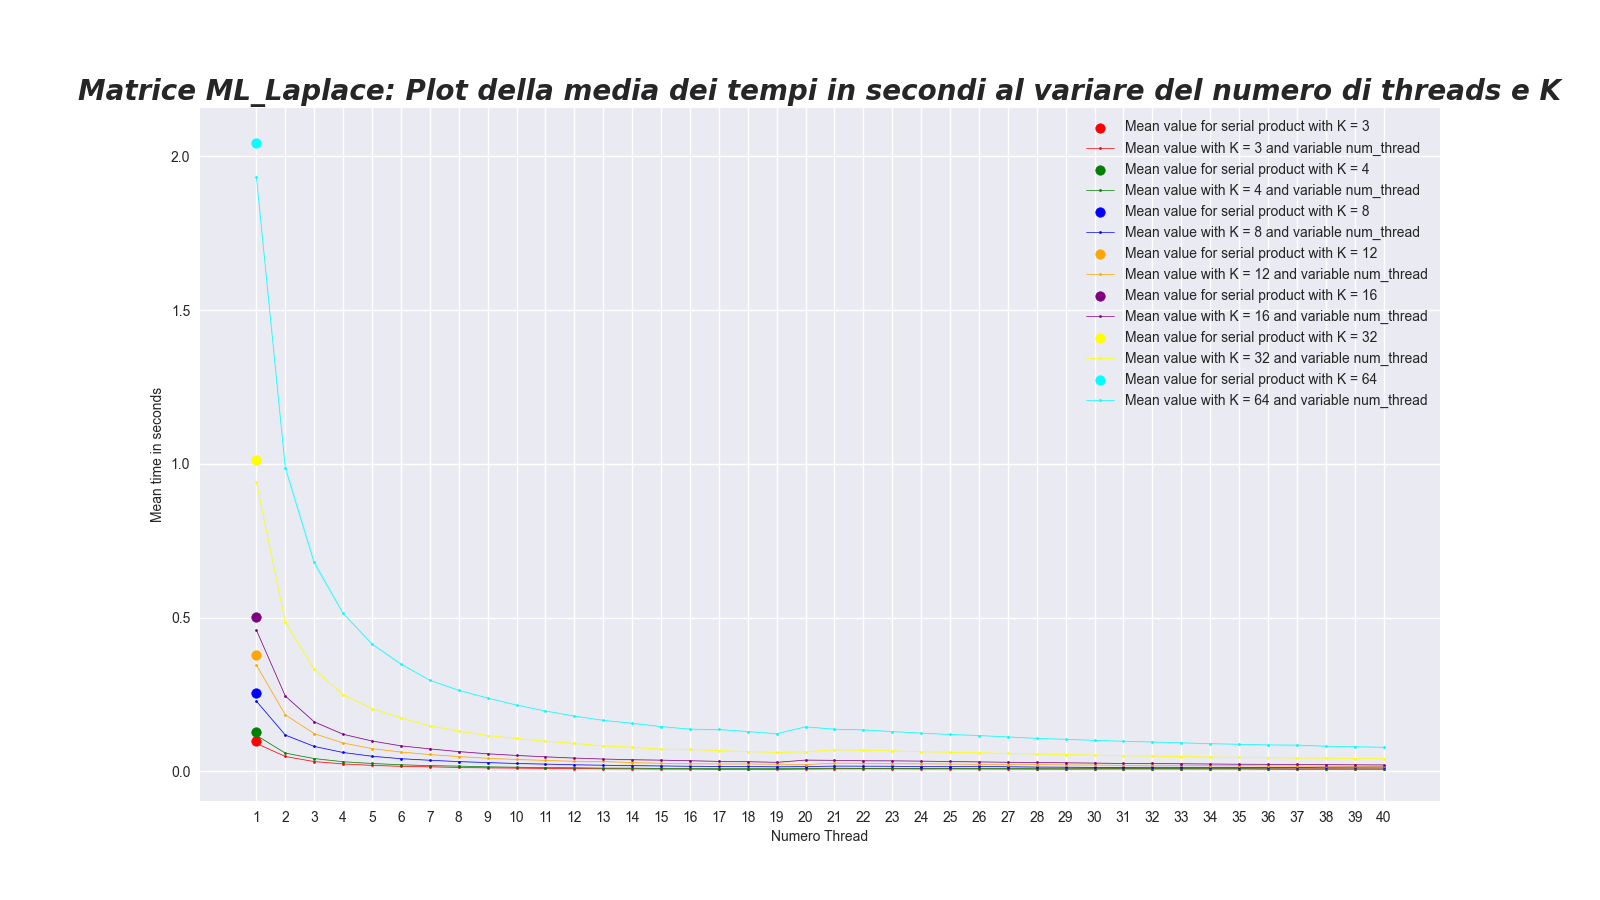
\includegraphics[width=\textwidth]{Immagini/CSR_CPU_ML_Laplace.png}
\caption{Tempi medi per la matrice ML\_Laplace nel formato CSR}
\end{figure}

Come da aspettative, abbiamo un grafico che è rispetto appieno il comportamento atteso. La spiegazione è molto intuitiva: 
\begin{itemize}
    \item  L'utilizzo di un numero maggiore di thread può sfruttare il parallelismo disponibile nel sistema, consentendo una maggiore distribuzione del carico di lavoro tra le unità di elaborazione. Quando il numero di thread aumenta, le attività possono essere eseguite contemporaneamente su più unità di elaborazione, riducendo il tempo complessivo di esecuzione. Tuttavia, è importante notare che l'aumento del numero di thread può comportare anche un sovraccarico aggiuntivo dovuto alla sincronizzazione e alla gestione dei thread stessi.
    \item L'aumento dei tempi medi al crescere del numero di colonne del multi-vettore (rappresentato da K) può essere attribuito a diversi fattori: 
    \begin{itemize}
        \item \textbf{Accesso alla memoria:} L'elaborazione di un multi-vettore richiede l'accesso a K elementi del vettore per ogni colonna della matrice. Quando K aumenta, aumenta anche la quantità di dati da leggere dalla memoria. Questo può comportare un maggior numero di cache misses, dove i dati richiesti non sono presenti nella cache e devono essere recuperati dalla memoria principale. L'accesso alla memoria principale è generalmente più lento rispetto alla cache, il che può influire negativamente sui tempi di esecuzione complessivi.
        \item \textbf{Dimensione dei dati:}  L'aumento del numero di colonne del multi-vettore comporta un aumento della dimensione complessiva dei dati coinvolti nell'operazione. Questo può influire sulla gestione della memoria, specialmente se la quantità di dati supera la capacità della cache o della memoria disponibile. L'aumento della dimensione dei dati può comportare un maggior numero di operazioni di trasferimento dati tra la memoria principale e la cache, che possono rallentare l'esecuzione complessiva dell'algoritmo.
    \end{itemize}
\end{itemize} 

Un andamento del tutto analogo (asintoticamente) si ha per la matrice adder\_dcop\_32, che rispetto al ML\_Laplace ha un numero medio di non zeri ($\frac{11.246}{1.813} \approx  6,202$ per adder\_dcop\_32  vs $\frac{27.689.972}{377.002} \approx  73,447$ per ML\_Laplace per riga notevolmente inferiore.  

\begin{figure}[H]
\centering
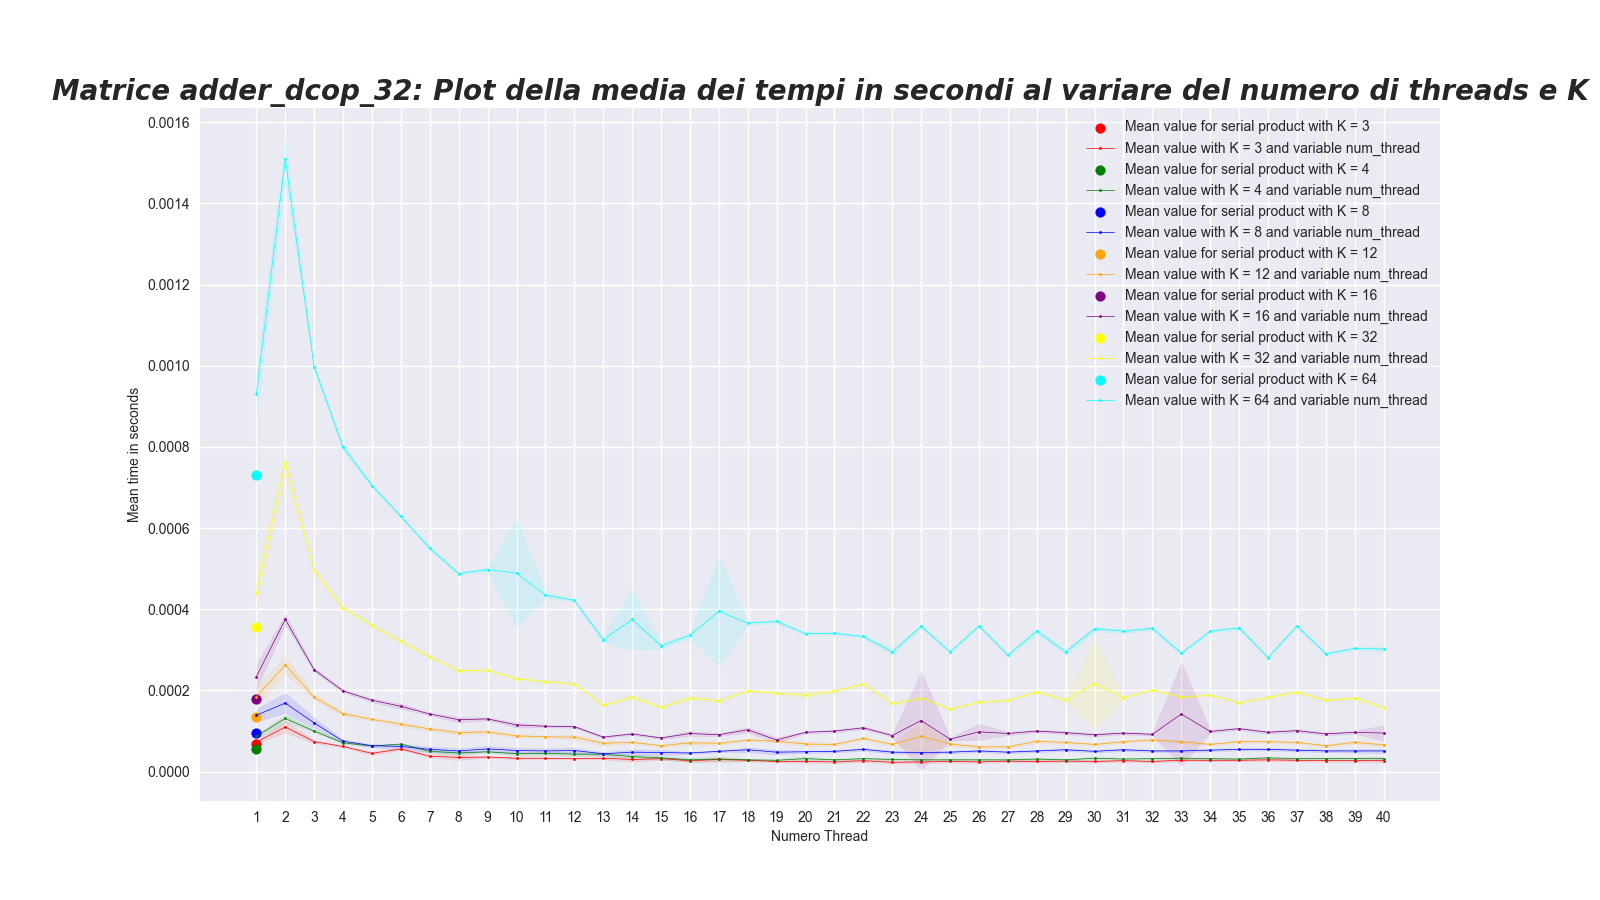
\includegraphics[width=\textwidth]{Immagini/CSR_CPU_adder_dcop_32.png}
\caption{Tempi medi per la matrice adder\_dcop\_32 nel formato CSR}
\end{figure}

\subsubsection{CPU e ELLPACK}

Per quanto riguarda il formato ELLPACK possiamo notare un comportamento analogo per entrambe le matrici precedenti.
\begin{figure}[H]
\centering
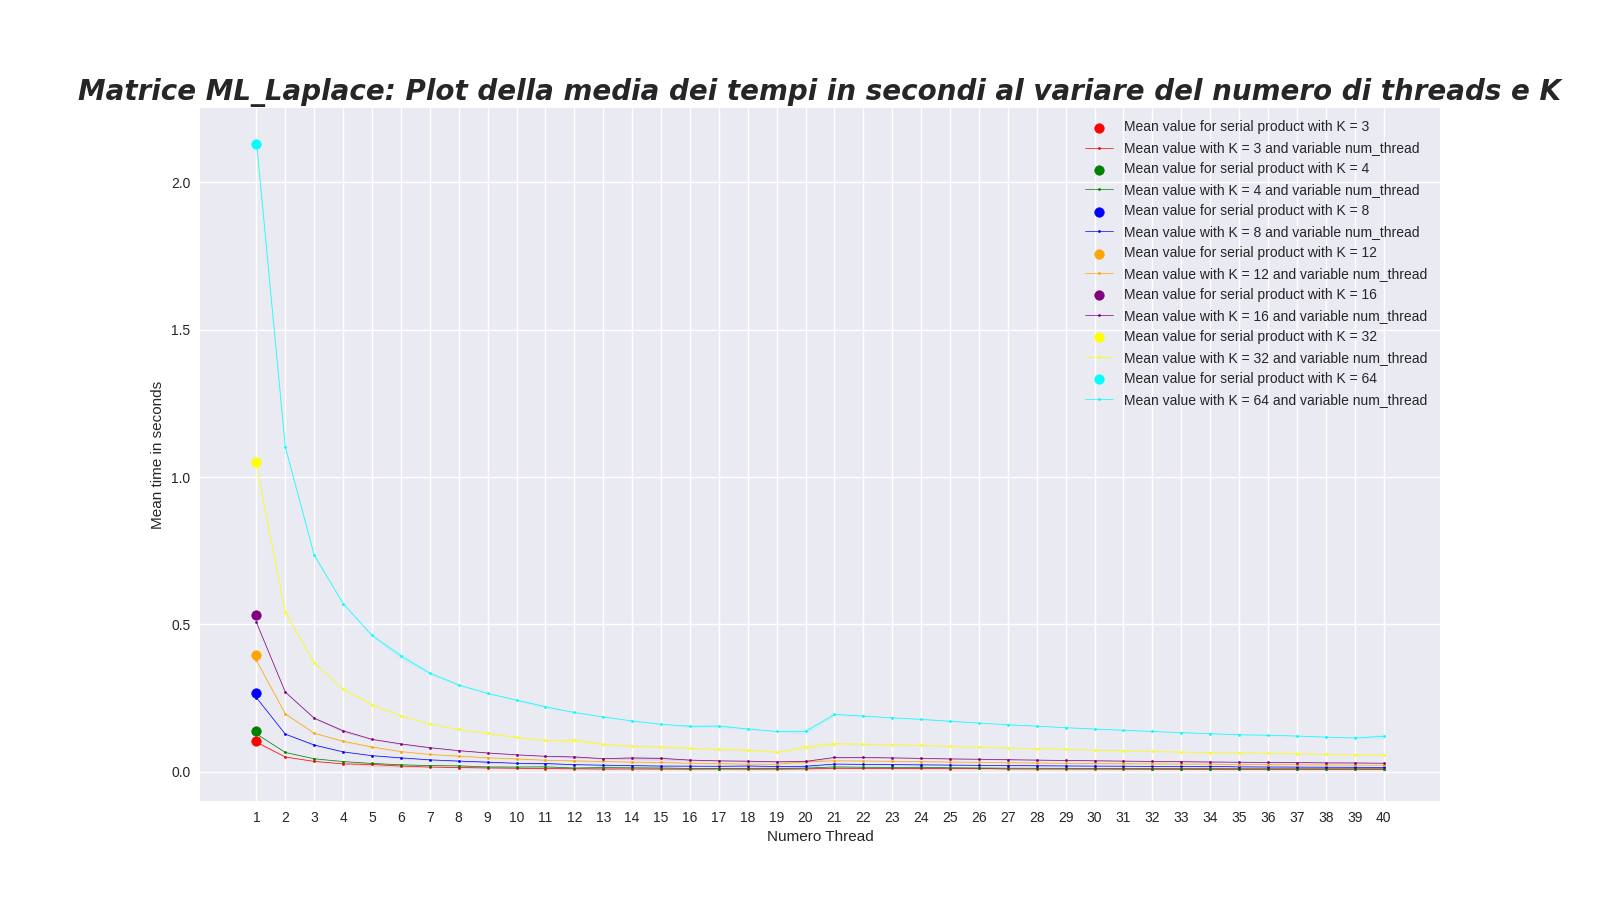
\includegraphics[width=\textwidth]{Immagini/ELLPACK_CPU_ML_Laplace.png}
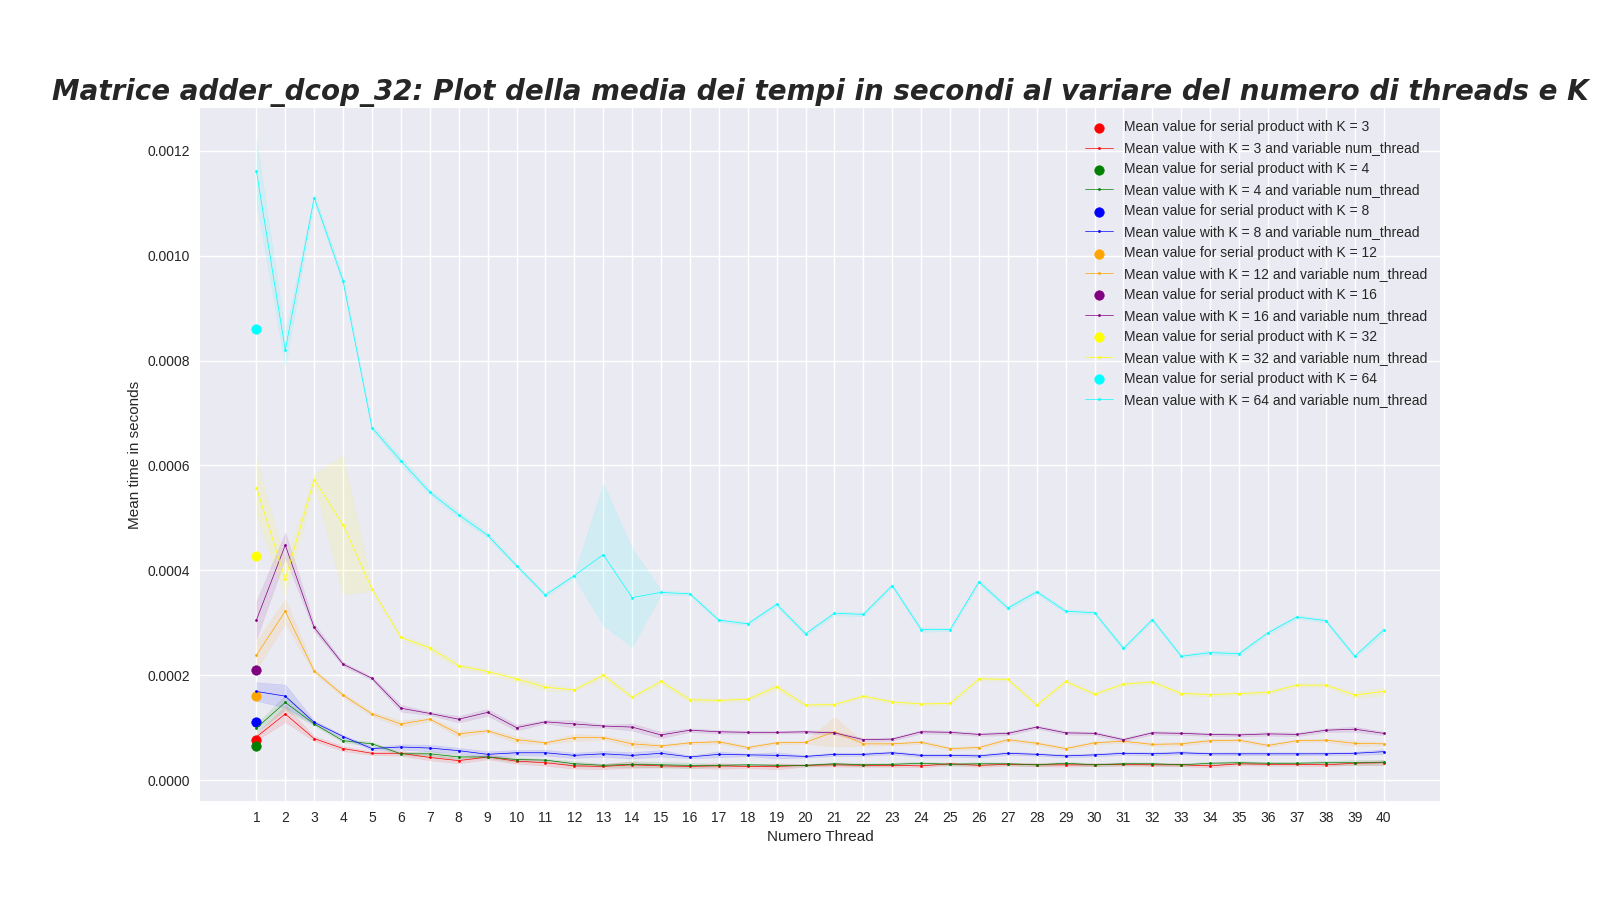
\includegraphics[width=\textwidth]{Immagini/ELLPACK_CPU_adder_dcop_32.png}
\caption{Tempi medi per la matrice ML\_Laplace e adder\_dcop\_32 nel formato ELLPACK}
\end{figure}

\subsection{Prestazioni su GPU}
La complessità intrinseca delle GPU ha reso difficile individuare un "pattern" ricorrente nelle trame dei prodotti matrice sparsa con multi-vettore. La GPU è un'architettura altamente specializzata progettata per eseguire in modo efficiente operazioni parallele su grandi quantità di dati. A differenza delle CPU, le GPU sono caratterizzate da un elevato grado di parallelismo massivo (quindi maggiore variabilità) e da una gerarchia di memoria complessa.\\

A causa di questa complessità, l'analisi delle prestazioni sulle GPU richiede un approccio dettagliato e specifico per l'architettura utilizzata. Le GPU moderne possono avere diverse generazioni, modelli e configurazioni, ognuna con le proprie caratteristiche uniche. Pertanto, è difficile identificare un pattern generale nei plots dei prodotti matrice sparsa con multi-vettore su GPU che sia applicabile a tutte le architetture.\\

Per quanto riguarda la GPU, abbiamo realizzato dei grafici che mostrano l'andamento medio dei GFLOPS al variare del kernel utilizzato e di K. Anche in questo caso abbiamo rappresentato la banda di confidenza del 95\%.
\\
\subsubsection{GPU e CSR}
Consideriamo per primo il formato CSR. Come detto in precedenza, per questo formato abbiamo realizzato diversi kernel. Per analizzarli conviene confrontare i risultati ottenuti per le matrici adder\_dcop\_32 e ML\_Laplace, essendo dimensionalmente e strutturalmente molto diverse.

\begin{figure}[H]
\centering
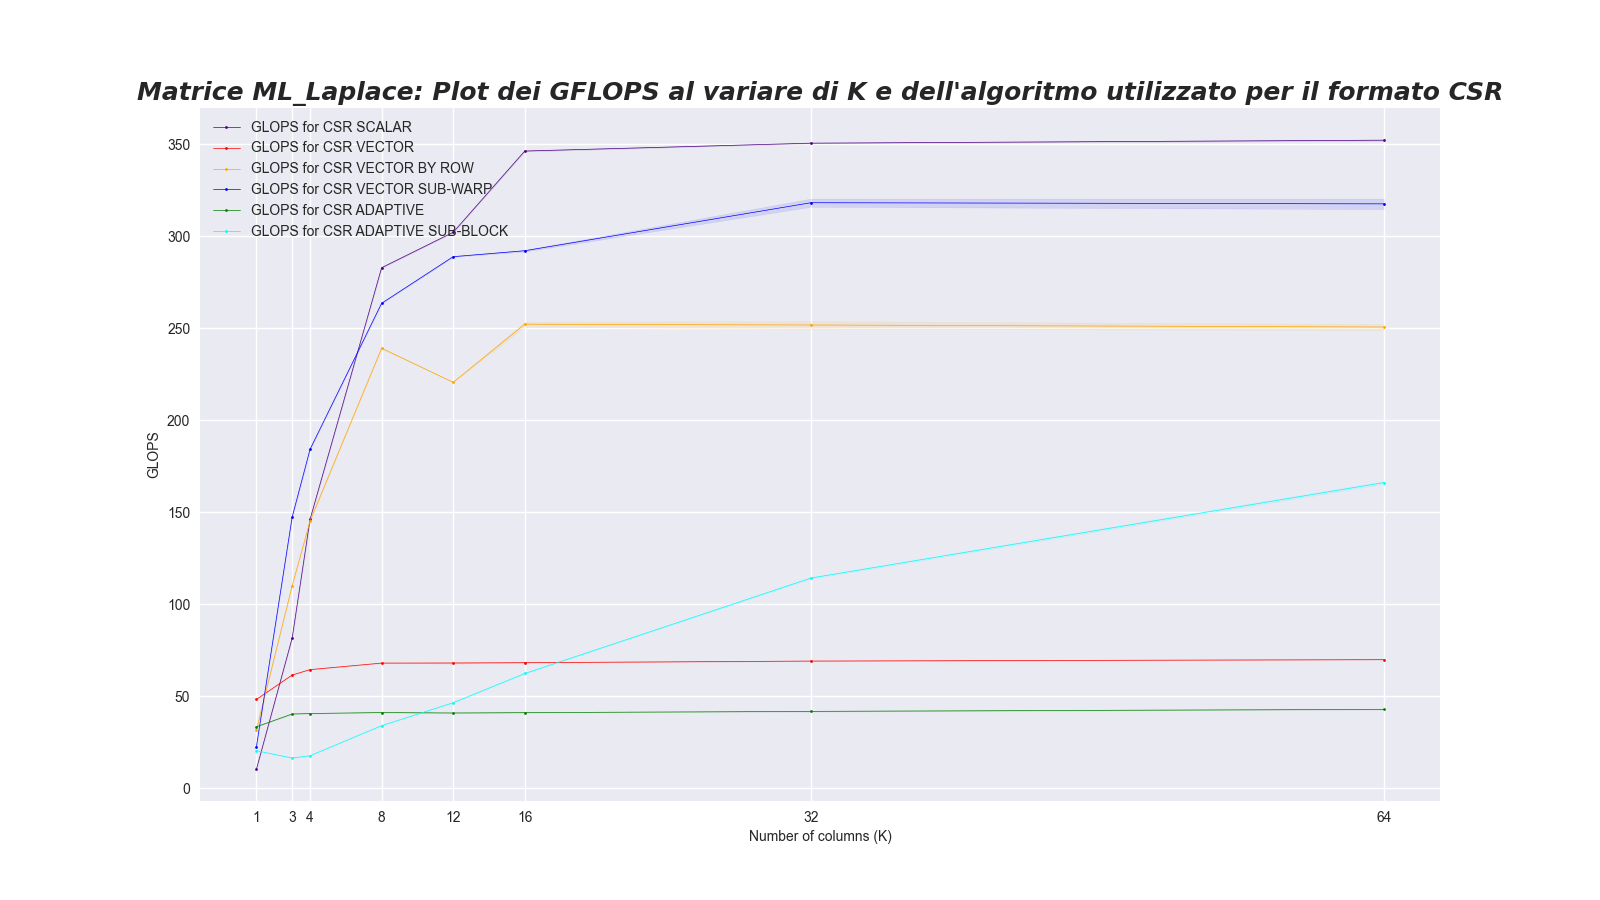
\includegraphics[width=\textwidth]{Immagini/CSR_GPU_ML_Laplace.png}
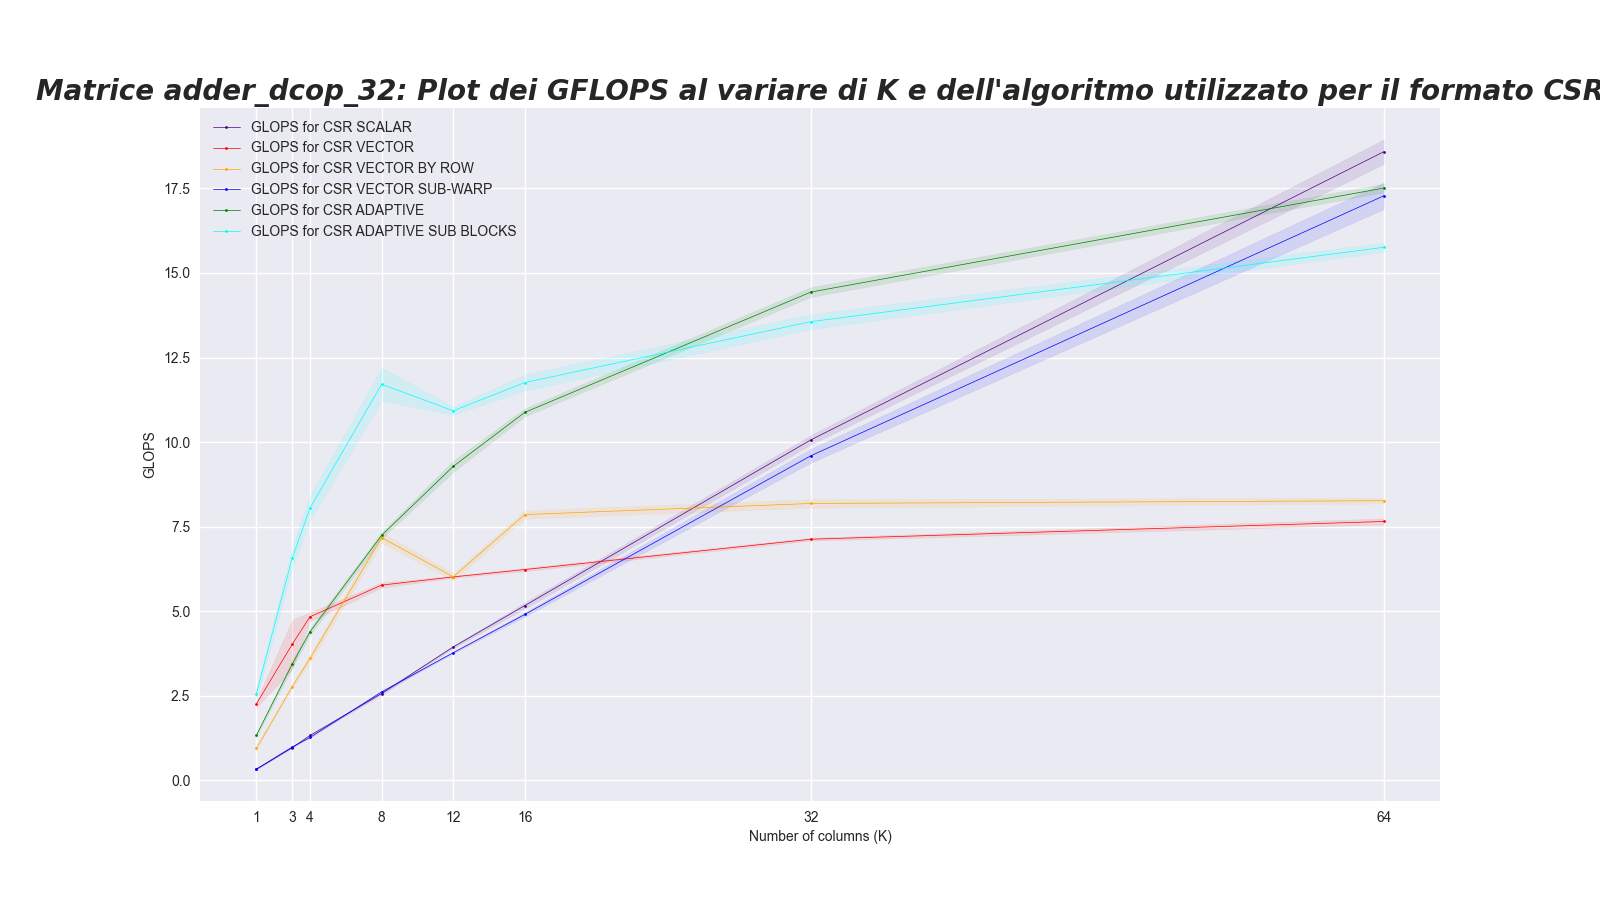
\includegraphics[width=\textwidth]{Immagini/CSR_GPU_adder_dcop_32.png}
\caption{GFLOPS per la matrice ML\_Laplace e adder\_dcop\_32 nel formato CSR}
\end{figure}

Un fattore determinante per analizzare le immagini precedenti è il numero medio di non zeri:
    \begin{itemize}
        \item  Per ML\_Laplace è $\frac{27.689.972}{377.002} \approx  73,447$
        \item Per adder\_dcop\_32 $\frac{11.246}{1.813} \approx 6,202$
    \end{itemize} 
    
E' possibile fare le seguenti considerazioni algoritmo per algoritmo:
(TODO)
\begin{itemize}
    \item \textbf{CSR\_SCALAR}
    \item \textbf{CSR\_VECTOR}
    \item \textbf{CSR\_VECTOR\_BY\_ROW}
    \item \textbf{CSR\_VECTOR\_SUB\_WARP}
    \item \textbf{CSR\_ADAPTIVE}
    \item \textbf{CSR\_ADAPTIVE\_SUB\_BLOCK}
\end{itemize}

\subsubsection{GPU e ELLPACK}
Per quanto riguarda il formato ELLPACK abbiamo la seguente situazione:
\begin{figure}[H]
\centering
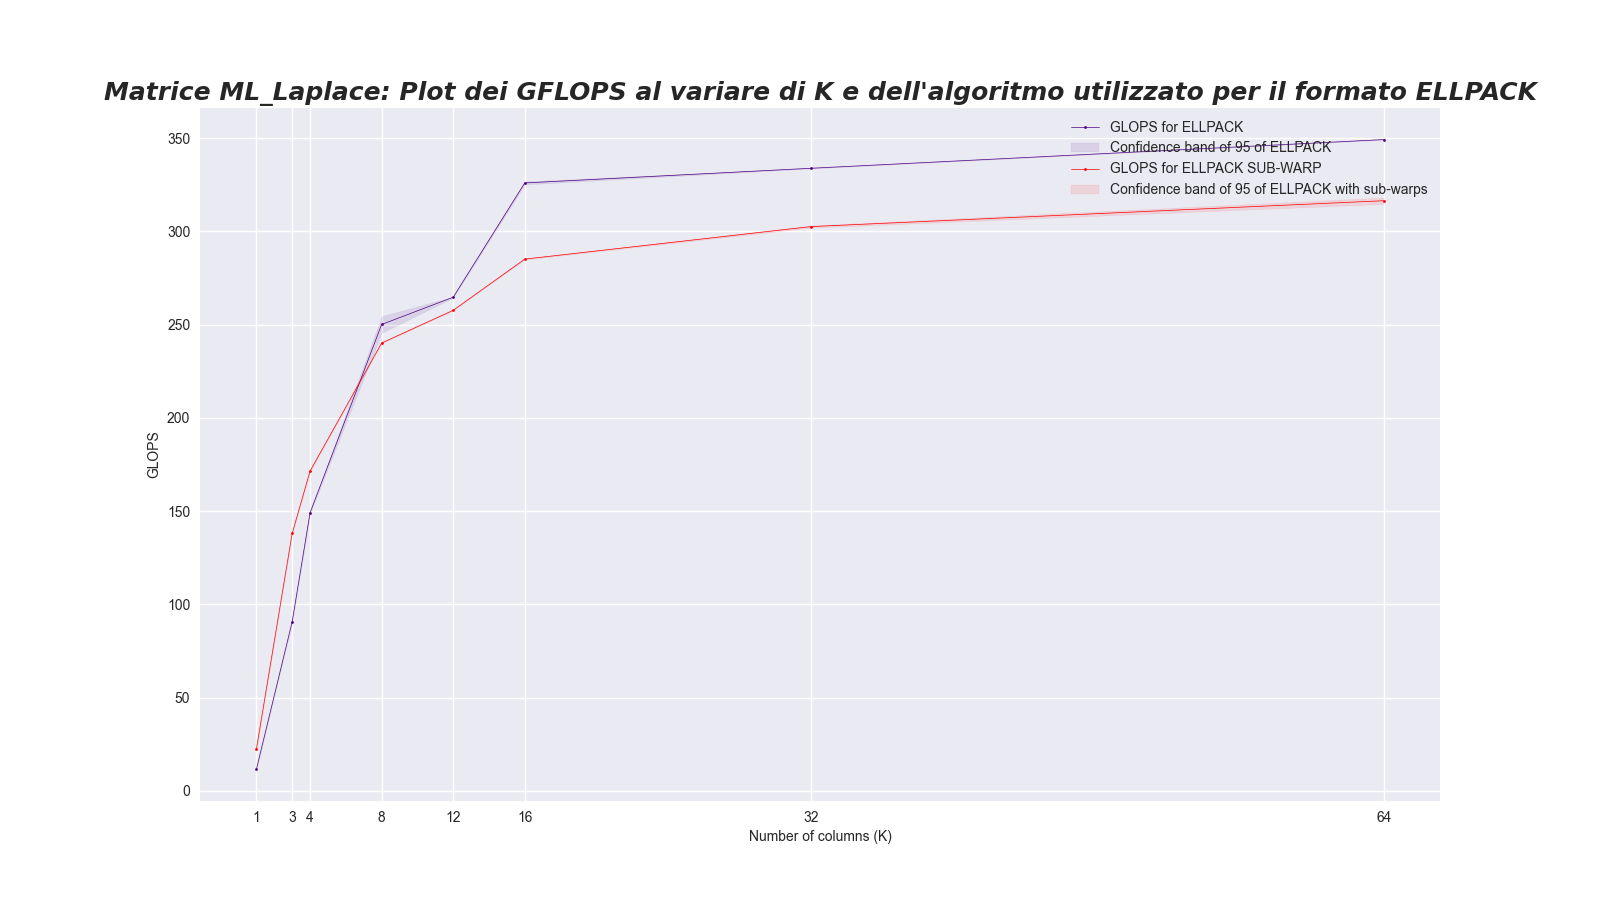
\includegraphics[width=\textwidth]{Immagini/ELLPACK_GPU_ML_Laplace.png}
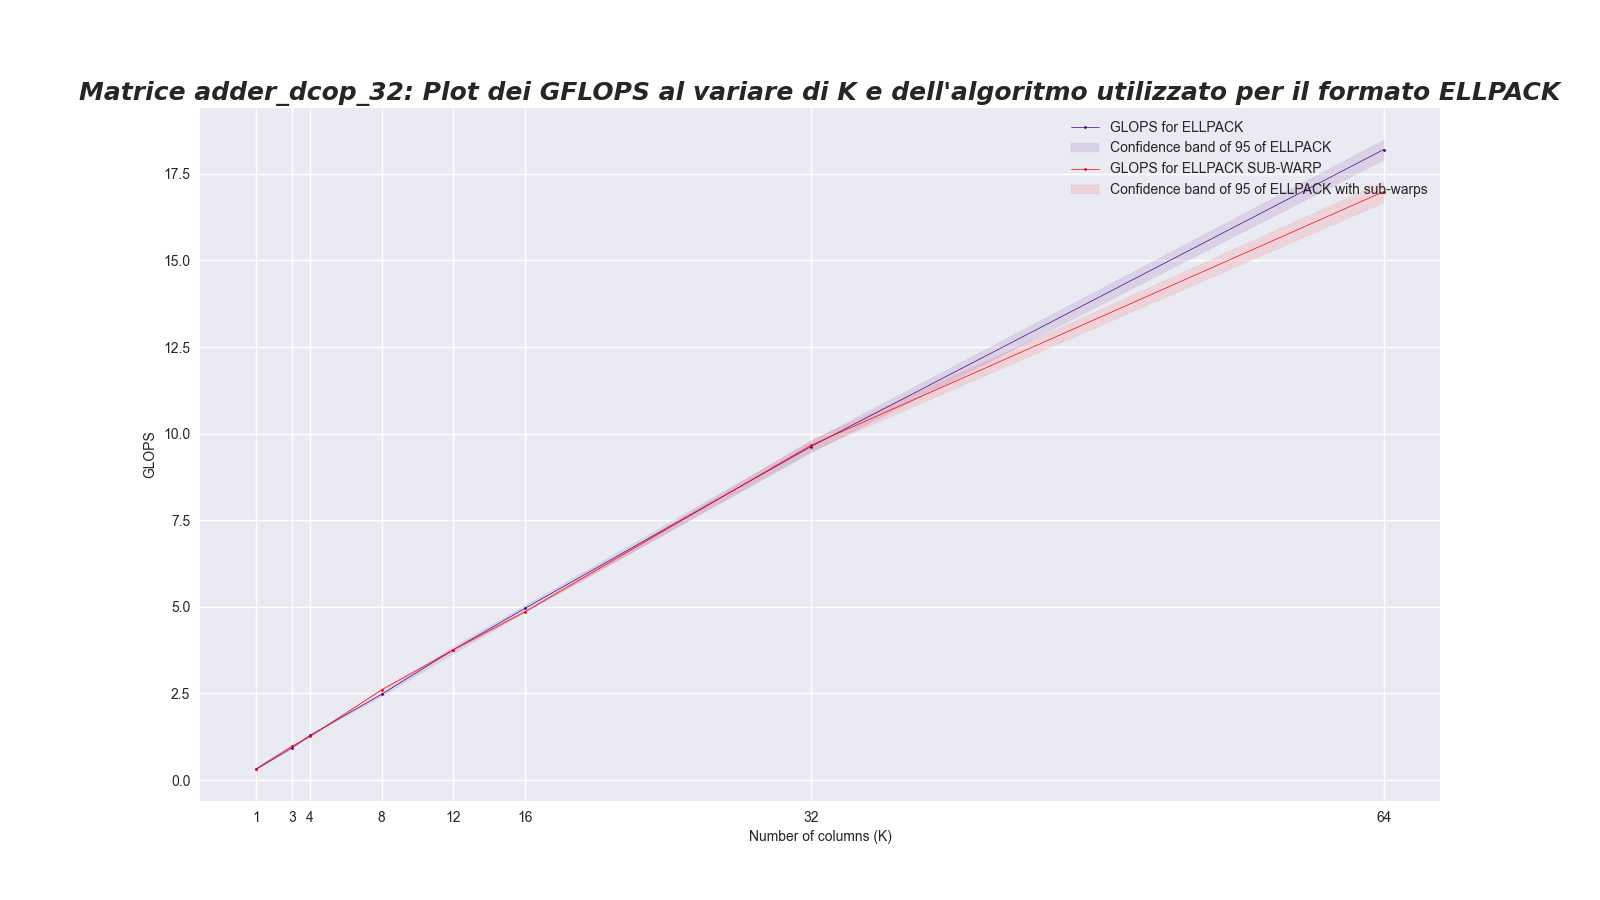
\includegraphics[width=\textwidth]{Immagini/ELLPACK_GPU_adder_dcop_32.png}
\caption{GFLOPS per la matrice ML\_Laplace e adder\_dcop\_32 nel formato ELLPACK}
\end{figure}

E' possibile fare le seguenti considerazioni algoritmo per algoritmo:
(TODO)
\begin{itemize}
    \item \textbf{ELLPACK\_SCALAR}
    \item \textbf{ELLPACK\_SUB\_WARP}
\end{itemize}

\section{Suddivisione del lavoro}
Il progetto è stato congiuntamente elaborato durante l'ultima sessione didattica. Di conseguenza, ci siamo incontrati giornalmente, dovendo seguire gli stessi corsi, per portare avanti il progetto e risolvere eventuali problematiche incontrate. Di fatto, non c'è una netta suddivisione del carico di lavoro.

\section{Istruzioni per la compilazione}
Per quanto riguarda la compilazione abbiamo reso disponibile nella root directory del progetto un Makefile. Il suo utilizzo può essere esemplificato nel seguente modo:
\begin{itemize}
    \item Compilazione openMP, a sua volta schematizzata nel seguente modo:
    \begin{itemize}
        \item \textbf{openmp-csr-compare-serial-parallel}: \begin{lstlisting}[style=bashstyle]
        #!/bin/bash
        make openmp-csr-compare-serial-parallel 
        \end{lstlisting} Con il precedente comando il codice viene compilato per eseguire sia il prodotto seriale che parallelo per il formato CSR, confrontare i tempi d'esecuzione e verificare la correttezza di quello parallelo attraverso un confronto elemento per elemento con quello seriale.
        \item \textbf{openmp-ellpack-compare-serial-parallel}  \begin{lstlisting}[style=bashstyle]
        #!/bin/bash
        make openmp-ellpack-compare-serial-parallel
        \end{lstlisting} Con il precedente comando il codice viene compilato per ottenere un eseguibile che calcoli sia il prodotto seriale che parallelo per il formato ELLPACK, confrontare i tempi d'esecuzione e verificare la correttezza di quello parallelo attraverso un confronto elemento per elemento con quello seriale.
        \item \textbf{openmp-csr-check-conversions}
         \begin{lstlisting}[style=bashstyle]
        #!/bin/bash
        make openmp-csr-check-conversions
        \end{lstlisting} Con il precedente comando il codice viene compilato per confrontare la conversione originale e quella ottimizzata dal formato COO al formato CSR.
        \item \textbf{openmp-ellpack-check-conversions}
        \begin{lstlisting}[style=bashstyle]
        #!/bin/bash
        make openmp-ellpack-check-conversions
        \end{lstlisting} Con il precedente comando il codice viene compilato per confrontare la conversione originale e quella ottimizzata dal formato COO al formato ELLPACK.
        \item \textbf{openmp-csr-serial-samplings}
         \begin{lstlisting}[style=bashstyle]
        #!/bin/bash
        make openmp-csr-serial-samplings
        \end{lstlisting} Con il precedente comando il codice viene compilato per ottenere un eseguibile che esegua al variare di K e del numero di thread, per SAMPLING\_SIZE volte il prodotto seriale, calcoli la media e la varianza dei tempi d'esecuzione in modo incrementale ed in un singolo passo attraverso l'algoritmo di (one-pass) Welford
        \item \textbf{openmp-ellpack-serial-samplings}
        \begin{lstlisting}[style=bashstyle]
        #!/bin/bash
        make openmp-ellpack-serial-samplings
        \end{lstlisting} Con il precedente comando il codice viene compilato per ottenere un eseguibile che esegua al variare di K e del numero di thread, per SAMPLING\_SIZE volte il prodotto seriale per il formato ELLPACK, calcoli la media e la varianza dei tempi d'esecuzione in modo incrementale ed in un singolo passo attraverso l'algoritmo di (one-pass) Welford
        \item \textbf{openmp-csr-parallel-samplings}
        \begin{lstlisting}[style=bashstyle]
        #!/bin/bash
        make openmp-csr-parallel-samplings
        \end{lstlisting} Con il precedente comando il codice viene compilato per ottenere un eseguibile che esegua al variare di K e del numero di thread, per SAMPLING\_SIZE volte il prodotto parallelo per il formato CSR, calcoli la media e la varianza dei tempi d'esecuzione in modo incrementale ed in un singolo passo attraverso l'algoritmo di (one-pass) Welford
        \item \textbf{openmp-ellpack-parallel-samplings}
        \begin{lstlisting}[style=bashstyle]
        #!/bin/bash
        make openmp-ellpack-parallel-samplings
        \end{lstlisting} Con il precedente comando il codice viene compilato per ottenere un eseguibile che esegua al variare di K e del numero di thread, per SAMPLING\_SIZE volte il prodotto parallelo per il formato ELLPACK, calcoli la media e la varianza dei tempi d'esecuzione in modo incrementale ed in un singolo passo attraverso l'algoritmo di (one-pass) Welford
    \end{itemize}
    
    \item Compilazione CUDA, a sua volta schematizzata nel seguente modo:
    \begin{itemize}
        \item \textbf{csr}
         \begin{lstlisting}[style=bashstyle]
        #!/bin/bash
        make all MODE=csr
        \end{lstlisting} Con il precedente comando si ottiene un eseguibile che lancia il prodotto seriale, il kernel CUDA \textit{CSR\_Scalar\_v3}, calcoli i GFLOPS e confronti il risultato del prodotto seriale con quello parallelo. 
        \item \textbf{csr\_adaptive}
          \begin{lstlisting}[style=bashstyle]
        #!/bin/bash
        make all MODE=csr_adaptive
        \end{lstlisting} Con il precedente comando si ottiene un eseguibile che lancia il prodotto seriale, il kernel CUDA \textit{CSR\_Adaptive}, calcoli i GFLOPS e confronti il risultato del prodotto seriale con quello parallelo. 
        \item \textbf{csr\_adaptive\_sub\_block}
        \begin{lstlisting}[style=bashstyle]
        #!/bin/bash
        make all MODE=csr_adaptive_sub_block
        \end{lstlisting} Con il precedente comando si ottiene un eseguibile che lancia il prodotto seriale, il kernel CUDA \textit{CSR\_Adaptive\_sub\_blocks}, calcoli i GFLOPS e confronti il risultato del prodotto seriale con quello parallelo. 
        \item \textbf{csr\_vector}
        \begin{lstlisting}[style=bashstyle]
        #!/bin/bash
        make all MODE=csr_vector
        \end{lstlisting} Con il precedente comando si ottiene un eseguibile che lancia il prodotto seriale, il kernel CUDA \textit{CSR\_Vector}, calcoli i GFLOPS e confronti il risultato del prodotto seriale con quello parallelo. 
        \item \textbf{csr\_vector\_by\_row}
        \begin{lstlisting}[style=bashstyle]
        #!/bin/bash
        make all MODE=csr_vector_by_row
        \end{lstlisting} Con il precedente comando si ottiene un eseguibile che lancia il prodotto seriale, il kernel CUDA \textit{CSR\_Vector\_by\_row}, calcoli i GFLOPS e confronti il risultato del prodotto seriale con quello parallelo. 
        \item \textbf{csr\_vector\_sub\_warp}
        \begin{lstlisting}[style=bashstyle]
        #!/bin/bash
        make all MODE=csr_vector_sub_warp
        \end{lstlisting} Con il precedente comando si ottiene un eseguibile che lancia il prodotto seriale, il kernel CUDA \textit{CSR\_Vector\_Sub\_warp}, calcoli i GFLOPS e confronti il risultato del prodotto seriale con quello parallelo. 
        \item \textbf{ellpack\_sw}
        \begin{lstlisting}[style=bashstyle]
        #!/bin/bash
        make all MODE=ellpack_sw
        \end{lstlisting} Con il precedente comando si ottiene un eseguibile che lancia il prodotto seriale, il kernel CUDA \textit{ELLPACK\_Sub\_warp}, calcoli i GFLOPS e confronti il risultato del prodotto seriale con quello parallelo. 
        \item \textbf{ellpack}
        \begin{lstlisting}[style=bashstyle]
        #!/bin/bash
        make all MODE=ellpack
        \end{lstlisting} Con il precedente comando si ottiene un eseguibile che lancia il prodotto seriale, il kernel CUDA \textit{ELLPACK\_kernel}, calcoli i GFLOPS e confronti il risultato del prodotto seriale con quello parallelo. 
    \end{itemize}

    \begin{itemize}
            \item[\Checkmark] \textbf{Senza campionamento}
         \begin{lstlisting}[style=bashstyle]
        #!/bin/bash
        make all SAMPLING=no
        \end{lstlisting} Con il precedente comando si ottiene un eseguibile che lancia il prodotto seriale, il kernel CUDA indicato nella variabile MODE (riga 19 nel Makefile), calcoli i GFLOPS e confronti il risultato del prodotto seriale con quello parallelo. 
        \item[\Checkmark] \textbf{Con campionamento}
        \begin{lstlisting}[style=bashstyle]
        #!/bin/bash
        make all SAMPLING=yes
        \end{lstlisting} Con il precedente comando si ottiene un eseguibile che lancia al variare di K, per SAMPLING\_SIZE volte, il kernel CUDA indicato nella variabile MODE (riga 19 nel Makefile), calcoli la media e la varianza GFLOPS in modo incrementale ed in un singolo passo attraverso l'algoritmo di (one-pass) Welford
    \end{itemize}
\end{itemize}

Una volta generato l'eseguibile \textit{app} nella directory \textit/all è possibile utilizzare nuovamente il comando make nel seguente modo:
 \begin{lstlisting}[style=bashstyle]
        #!/bin/bash
        make ML_Laplace 
\end{lstlisting}. 
        
    In questo caso viene avviato il programma con in input la matrice ML\_Laplace.

\section{Struttura del codice e sua riutilizzabilità}
Il codice è organizzata nelle seguenti directory:
\begin{itemize}
    \item \textit{CUDA}: In questa directory sono presenti 3 files :
    \begin{itemize}
        \item \textit{parallel\_product\_CSR.cu}: Contiene la funzione di setup e il codice sorgente dei kernel per il formato CSR.
        \item \textit{parallel\_product\_ELLPACK.cu}:
        Contiene la funzione di setup e il codice sorgente dei kernel per il formato ELLPACK.
        \item \textit{samplings.cu}:
        Contiene le funzioni implementare per effettuare il sampling per il nucleo di calcolo realizzato in CUDA.
    \end{itemize}
    \item \textit{doc}: E' la directory che contiene la relazione e le immagini utilizzate per realizzarla.
    \item \textit{include}: E' la directory che contiene gli headers.
    \item \textit{lib}: E' la directory che contiene la libreria ausiliaria \textit{mmio.c} 
    \item \textit{openMP}:
     In questa directory sono presenti 3 files :
    \begin{itemize}
        \item \textit{parallel\_product.c}: Contiene i codici che implementano i prodotti paralleli in openMP per il formato ELLPACK e CSR.
        \item \textit{samplings.c}:
         Contiene le funzioni implementare per effettuare il sampling per il nucleo di calcolo realizzato in openMP.
    \end{itemize}
    \item \textit{plots}: E' la directory che contiene i file python realizzati per sviluppo dei grafici, i plot nel formato .png e i file CSV con il risultato del campionamento. 
\end{itemize}

Nella directory root, quella più "esterna" abbiamo i seguenti files:
\begin{itemize}
    \item \textit{checks.c}: Contiene le funzioni necessarie per effettuare i controlli sulla correttezza delle conversioni e del prodotto parallelo.
    \item \textit{conversions\_parallel.c}: E' presente il codice sviluppato per realizzare le conversioni in modo parallelo dal formato COO al formato CSR ed ELLPACK.
    \item \textit{conversions\_serial.c}
    E' presente il codice sviluppato per realizzare le conversioni in modo seriale dal formato COO al formato CSR ed ELLPACK.
    \item \textit{create\_mtx\_coo.c}: Sono presenti le funzioni che implementano la lettura del file .mtx e conseguente allocazione di memoria per memorizzare la matrice nel formato COO.
    \item \textit{main.c}: E' il file che contiene il main, che si comporta come orchestratore del programma.
    \item \textit{Makefile}: E' il Makefile descritto nella sezione precedente.
    \item \textit{serial\_product.c}: Contiene le funzioni implementate per realizzare il prodotto seriale per il formato CSR ed ELLPACK.
    \item \textit{utils.c}: Contiene le funzioni di utilità implementate. 
\end{itemize}

\end{document}